%!TEX root = main.tex


Here I argue that correctly applying the framework of causal Bayesian networks requires consideration of the decision set $D$ underwriting any decision problem, which is forced in CSDT.

\section{The switch and lightbulb}

\begin{quote}
	There is a lightbulb and a switch (maybe there are other things as well). We have a set $D$ of actions available, some of which we know turn the switch on and the rest of which we know turn the switch off, but the effect of any action on the lightbulb is uncertain. We have a very large number $N$ of IID observations of the joint state of the lightbulb and switch. We are interested in choosing decisions that control the light.
\end{quote}

This problem exhibits a number of features which we take to be common to any statistical causal decision problem:
\begin{itemize}
	\item There is a set of decisions, known in advance, that may be chosen
	\item We possess some incomplete prior knowledge about the effects of decisions
	\item Data is available (observations of the switch and light state)
	\item The objective is to control some feature of the environment
\end{itemize}

This is a general problem, and there are many different observations and consequence maps compatible with it. For example, we might have:
\begin{itemize}
	\item The switch always turns the light on both in observations and as a result of our actions (more precisely, the switch and light always share the same state in observations and for all actions)
	\item In observations the light is on iff the switch is on, some actions preserve this relationship (``just turn the light on'') while some break it (``cut power to the house, turn the light on'')
	\item There is another switch (``switch 2'') in the house which also controls the light which is randomly on or off in observations. Thus in observations the light is uncorrelated with switch 1 but there are nevertheless actions available that control the light: ``turn switch 2 off, then turn switch 1 on'' (there is, however, no way of concluding that this would work without making additional assumptions)
\end{itemize}

Consider a version of this problem with two additional assumptions: (1) the actions available are sufficient to reproduce the observed joint behaviour of $(switch,light)$ and (2) there is only 1 way to switch the light off and 1 way to switch it on (i.e. $|D|=2$). In this case the observed behaviour of the light conditional on the switch's state must be the behaviour of the light under the unique ``off'' and ``on'' actions. Suppose we instead assume (2') there is only 1 way to switch the light off and there are 2 ways to switch it on (let's call them $d_1$ and $d_2$). In this case we can still determine the behaviour of the light from observations when we turn the switch off, but we cannot determine as much when we switch it on - the best that we can say is that some mixture of $d_1$ and $d_2$ will reproduce the observed behaviour of the light when the switch is on. This doesn't limit the behaviour of the light under $d_1$ or $d_2$ individually - if we observe the light was on every time the switch was on, but this was always the result of taking $d_2$, then it is perfectly possible that $d_1$ never switches the light on. On the other hand, if we always observe the light is on when the switch is on, then a random action that takes $d_1$ half the time and $d_2$ half the time must leave the light on at least half the time.

\subsection{Using Causal Theories}

To model this situation with a causal theory, we need to define the Markov kernel representing the coupled observation model $\mathscr{H}:\Theta\to \Delta(\{0,1\}^2)$ and consequence model $\mathscr{C}:\Theta\times D\to \Delta(\{0,1\}^2)$. The latent space $\Theta$ represents the set of coupled models we consider to be possible.

If we make no assumptions beyond what was specified in the original problem, our observatonal model should admit every possible distribution in $\Delta(\{0,1\})^2$. We have assumed that some decisions are known to turn the switch on and some turn the switch off. Let decisions be enumerated with an integer index $j$, and suppose $d_j\in D$ is a decision that turns the switch off iff $j<=0$. That is, we have

\begin{align}
\mathscr{C}_{\RV{S}_c|\RV{D}} = \begin{cases}
d_j \mapsto \delta_1 & j>0\\
d_j \mapsto \delta_0 & j<=0
\end{cases}
\end{align}

The ``post-decision'' state of the light $\RV{L}_c$ conditioned on the switch $\RV{S}_c$ and the decision $\RV{D}$ is given by $\mathscr{C}_{\RV{L}_c|\RV{S}_c\RV{D}}$ and like the observations is unrestricted. We've also made no assumptions about how observations go with consequences, each possible observational distribution will go with each possible consequence.

Thus $\Theta$ must represent the cartesian product of the set of observational distributions $\Delta(\{0,1\}^2)$ and set of possible conditionals $\mathscr{C}_{\RV{L}_c|\RV{S}_c\RV{D}}$. We can represent the latter set as $[0,1]^{2|D|}$ - the distribution of the binary $\RV{L}_c$ can be parametrised by $p\in [0,1]$, and each possible model assigns a particular parameter $p_{d_j}\in [0,1]$ to each $d_j\in \RV{D}$, giving $\Theta = \Delta(\{0,1\}^2)\times [0,1]^{2|D|}$.

Beyond the basic assumption that the behaviour of the light and switch can be represented by a Markov kernel, we add the assumption that $D$ is countable. Otherwise, we have as far as possible represented just the information given, and we conclude (as we ought to from the original setup) that we do not possess sufficient information to control the light - whatever observations we make, we admit the possibility of arbitrary $\mathscr{C}_{\RV{L}_c|\RV{S}_c\RV{D}}$.

We can also model the controllable case. For example, suppose $|D| = 2$, with one decision that turns the switch off and one that turns it on (decisions may still have side effects, but this rules out the possibility that there may be two decisions that turn the switch off each with \emph{different} side effects). Suppose also that the problem is \emph{reproducible} - that is, there is some stochastic action $\gamma\in \Delta(\mathcal{D})$ such that $\gamma \mathscr{C}_{\RV{L}_c\RV{S}_c|\RV{D}} = \mathscr{H}_0$. Then it follows that $\mathscr{C}_{\RV{L}_c|\RV{S}_c\RV{D}} = \mathscr{H}_{\RV{L}_o|\RV{S}_o}\otimes \stopper{0.25}_D$ and so the light may be controlled to the extent permitted by $\mathscr{H}_{\RV{L}_o|\RV{S}_o}$.

If we suppose that there are two decisions that turn the switch on - $d_1$ and $d_2$ - then we can derive inequality constraints on the consequences of mixtures of $d_1$ and $d_2$. Fix a state $\theta^*\in\Theta$ and let $p_{(on)}:= \mathscr{H}^{\theta^*}_{\RV{L}_o|\RV{S}_o}(1;\{1\})$ be the observed probability that the light is on given that the switch is on. Then given the mixed decision $\gamma=a \delta_{d_1} + (1-a)\delta_{d_2}$ and supposing $a>0.5$, we can say that 

\begin{align}
\mathrm{min}(0,p_{(on)}-a) \leq (\gamma\mathscr{C}^{\theta^*})_{\RV{L}_c|\RV{S}_c} \leq \mathrm{max}(1,p_{(on)}+a) \label{eq:three_decisions}
\end{align}


\subsection{Using Causal Bayesian Networks}

In order to approach this problem using causal Bayesian networks we must represent our assumptions in a graph $\mathcal{G}$ over some set of variables, and we must furthermore provide a \emph{do-scheme}, which is a map from the set of decisions $D$ provided by the problem. I am not aware of a set of instructions anywhere about how this ought to be done, and as we will see the process of doing so is less straightforward than one might expect.

It is possible to model causal theories using causal Bayesian networks where the ``state of the world'' $\theta$ is left implicit. We have posited a decision that can influence the state of a switch and a light. If we propose causal random variables $\RV{D}$, $\RV{S}$ and $\RV{L}$ corresponding to decision, switch and light respectively, then we might turn this sentence into the following diagram, with the understanding that interventions may only apply to the node labeled ``$\RV{D}$'':

\begin{align}
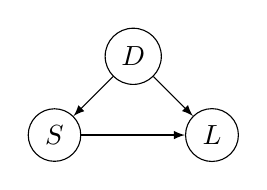
\begin{tikzpicture}[-latex]
\path (0,0) node[draw,circle] (D) {$\RV{D}$}
++(-1,-1) node[draw,circle] (S) {$\RV{S}$}
++(2,0) node[draw,circle] (L) {$\RV{L}$};
\draw (D) -- (S);
\draw (S) -- (L);
\draw (D) -- (L);
\end{tikzpicture}\label{dia:d_influences_both}
\end{align}

We will also formally specify a \emph{do-scheme} $f$ that relates the decisions available $D$ to $do(..)$ interventions on a given DAG. In this case, the do-scheme is straighforward. For a set of random varaiable $A$ Define $\mathrm{Do}_{A}$ to be the set of all statements of the form $do(\RV{X}_i=a,X_j=b)$ for $\{\RV{X}_i,\RV{X}_j\}\subset A$, $a\in \mathrm{Range}(\RV{X}_i)$, $b\in \mathrm{Range}(\RV{X}_j)$. Then the do-scheme $f:D\to \mathrm{Do}_{\{\RV{D}\}}$ is given by

\begin{align}
	f(a) := do(\RV{D}=a) \label{eq:do_scheme_trivial}
\end{align}

Diagram \ref{dia:d_influences_both} and do-scheme \ref{eq:do_scheme_trivial} corresponds to a causal theory with \emph{reproducibility}. To see this, observe that the graph represents two things. First, we have via the do-scheme that $\mathscr{C} = P(\RV{S},\RV{L}|do(\RV{D}))$ - i.e. the ``interventional map'' is the consequence map for the given problem. Secondly, it asserts that the observed joint distribution of $\RV{S}$ and $\RV{L}$ is the product of the conditional $P(\RV{S},\RV{L}|\RV{D})$ (which may be an arbitrary kernel of the appropriate type) and a latent marginal $\gamma_{\RV{D}}\in \Delta(\mathcal{D})$ (which may also be an arbitrary measure of the appropriate type). Note also that in this case $P(\RV{S},\RV{L}|\RV{D})=P(\RV{S},\RV{L}|do(\RV{D}))=\mathscr{C}$. Thus it asserts that the observational distribution is given by $\gamma_{\RV{D}}\mathscr{C}$ for some $\gamma_{\RV{D}}\in \Delta(\mathcal{D})$ - this is precisely the assumption of reproducibility, and as noted no other assumptions have been made.

If we want to posit a non-reproducible theory using DAGs, we would need to construct two ``parallel DAGs'':

\begin{align}
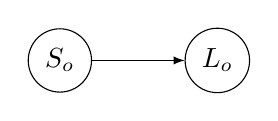
\begin{tikzpicture}[-latex]
\path (0,0) node[draw,circle] (S) {$\RV{S}_o$}
++(2,0) node[draw,circle] (L) {$\RV{L}_o$};
\draw (S) -- (L);
\end{tikzpicture} \qquad
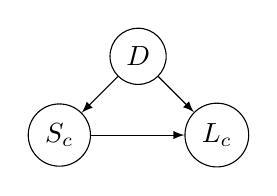
\begin{tikzpicture}[-latex]
\path (0,0) node[draw,circle] (D) {$\RV{D}$}
++(-1,-1) node[draw,circle] (S) {$\RV{S}_c$}
++(2,0) node[draw,circle] (L) {$\RV{L}_c$};
\draw (D) -- (S);
\draw (S) -- (L);
\draw (D) -- (L);
\end{tikzpicture}\label{dia:d_influences_both_nonreproducible}
\end{align}

Compare this to the graphical representation of the corresponding causal theory, and I hope it is clear how the two diagrams are related with the key difference being the explicit representation of the joint $\theta$ dependence in the causal theory as well as explicit representation of the Markov kernel

\begin{align}
\begin{tikzpicture}
\path (0,0) node (T) {$\theta$}
+(0,-1.15) node (D) {$\RV{D}$}
++ (0.3,0) coordinate (copy0)
++ (0.5,0) node[kernel] (H) {$\mathscr{H}$}
+ (0,-1) node[kernel] (C) {$\mathscr{C}$}
++ (0.7,0.15) node (So) {$\RV{S}_o$}
+ (0,-0.3) node (Lo) {$\RV{L}_o$}
+ (0,-1.) node (Sc) {$\RV{S}_c$}
+ (0,-1.3) node (Lc) {$\RV{L}_c$};
\draw (T) -- (H) ($(H.east) + (0,0.15)$) -- (So) ($(H.east)+(0,-0.15)$) -- (Lo);
\draw (copy0) to [bend right] ($(C.west)+(0,0.15)$) (D) -- ($(C.west)+(0,-0.15)$);
\draw ($(C.east) + (0,0.15)$) -- (Sc) ($(C.east)+(0,-0.15)$) -- (Lc);
\end{tikzpicture}
\end{align}

Diagrams \ref{dia:d_influences_both} and \ref{dia:d_influences_both_nonreproducible} along with the trivial do-scheme \ref{eq:do_scheme_trivial} show how we can represent causal theories using CBNs. These are unusual CBNs, though - for example, the arrow representing ``causal relationship'' between $\RV{S}$ and $\RV{L}$ could be reversed with no effect on the inference problem. In addition, the ``intervenable'' variable $\RV{D}$ is censored in the observations. As we have shown, identification is still possible given additional assumptions - partial prior knowledge, reproducibility and a sufficiently small set $D$.

However, we might also ask when it is possible to represent the inference problem using a more typical sort of DAG. Consider the case where we have both reproducibility and $|D|=2$. In this case, the relevant causal theory can be shown to correspond precisely to the CBN given by
\begin{align}
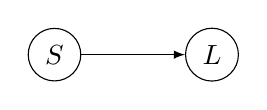
\begin{tikzpicture}[-latex]
\path (0,0) node[draw,circle] (S) {$\RV{S}$}
++(2,0) node[draw,circle] (L) {$\RV{L}$};
\draw (S) -- (L);
\end{tikzpicture}\label{dia:s_causes_l}
\end{align}

when equipped with the do-scheme $f:D\to \mathrm{Do}_{\{\RV{S},\RV{L}\}}$:
\begin{align}
f : \begin{cases}
	d_0 \mapsto \mathrm{do}(\RV{S}=0)\\
	d_1\mapsto \mathrm{do}(\RV{S}=1)
\end{cases}\label{eq:swl_do_scheme}
\end{align}

Here we also adopt the convention of assuming that the codomain of the do-scheme is the set of every variable represented on the graph (even though we do not make use of this full codomain).

The example was setup to suggest this interpretation. I also belive that in the controllable case, proponents of the CBN approach are likely to agree that
\begin{enumerate}
 \item The DAG \ref{dia:s_causes_l} is an appropriate representation of the causal structure of the switch-light example
 \item The two actions available do indeed correspond to $do(\RV{S}=0)$ and $do(\RV{S}=1)$; in other words, the do-scheme \ref{eq:swl_do_scheme} is appropriate
\end{enumerate}

That is, I am not just claiming that \ref{dia:s_causes_l} and \ref{eq:swl_do_scheme} is appropriate because it happens to yield the correct causal theory - it is also likely to be judged appropriate by anyone who takes the view that CBNs as typically used are appropriate tools for addressing causal inference problems.

Consider now the case where there are two ways to turn the light on and only one way to turn it off. In this case there is no do-scheme on diagram \ref{dia:s_causes_l} that yields the inequality \ref{eq:three_decisions} as the sole constraint on the results of mixtures of $d_1$ and $d_2$. This is true even if we allow:
\begin{itemize}
	\item Compound $do(..)$ statements like $do(\RV{S}=1,\RV{L}=0)$
	\item The passive $do()$ statement that yields the same distribution over $\RV{S}$ and $\RV{L}$ as was observed
	\item Conditional $do(..)$ operations; e.g. define $g:\{0,1\}\to \{0,1\}$ and let $do(\RV{S}=1,\RV{L}=g(\RV{S}))$ be defined as the operation that sets $\RV{S}=1$ and $\RV{L}=\RV{S}$ 
	\item Stochastic do-schemes e.g. $f(d_0) = 0.25(\delta_{do(\RV{S}=1)} + \delta_{do(\RV{S}=1,\RV{L}=0)} + \delta_{do()} + \delta_{do(\RV{S}=1,\RV{L}=g(\RV{S}))})$
\end{itemize}
This is a consequence of the fact that, for a discrete space $D$ and fixed the observational distribution, Causal Bayesian Networks assign a unique consequence to each action (the effects of interventions are all identifiable).

The notion that diagram \ref{dia:s_causes_l} ``correctly represents the causal relationships of the problem'' seems to be true when $|D|=2$ and we are prepared to assume reproducibility, but not when $|D|>=3$. This example shows that the construction of causal graphs depends on the set of actions available. One can also make this argument in terms of causal relationships: if we expect decisions to effect interventions on causally relevant unobserved variables, then the appropriate graph should contain these variables, whereas there is no need to include them if we expect decisions to effect interventions only on observed variables. I don't know if this is a generally accepted proposition, but I have not seen it mentioned in the CBN literature.

A related observation \emph{is} found in the potential outcomes literature:

\begin{quote}
 SUTVA [...] assumes that there are no hidden versions of treatments; no matter how unit i received treatment 1, the outcome that would be observed would be Y i (1) and similarly for treatment 0 \citep{rubin_causal_2005}
\end{quote}

\subsection{Does smoking cause cancer?}

\citet{pearl_does_2018} has used the example of smoking causing cancer in defense of the notion of ``causal relationships'' over ``consequences of given actions'':

\begin{quote}
Smoking cannot be stopped by any legal or educational means available to us today; cigarette advertising can. That does not stop researchers from aiming to estimate “the effect of smoking on cancer,” and doing so from experiments in which they vary the instrument -- cigarette advertisement -- not smoking.  The reason they would be interested in the atomic intervention $P(cancer|do(smoking))$ rather than (or in addition to) $P(cancer|do(advertising))$ is that the former represents a stable biological characteristic of the population, uncontaminated by social factors that affect susceptibility to advertisement, thus rendering it transportable across cultures and environments. With the help of this stable characteristic, one can assess the effects of a wide variety of practical policies, each employing a different smoking-reduction instrument
\end{quote}

The claim that Pearl is making here is at least an approximate version of the following:
\begin{enumerate}
	\item Public health workers have a large set $|D|$ of decisions that may affect the incidence of smoking. Represent smoking with $\RV{S}$, taking values in $\{0,1\}$
	\item Smoking has its own ``effect'' on rates of cancer. Represent cancer incidence with $\RV{R}$, taking values in $\{0,1\}$, and smoking's efffect with $\mathscr{C}_{\RV{R}|\RV{S}}:\{0,1\}\to \Delta(\{0,1\})$
	\item If we by some means acquire knowledge of the effect of decisions on the incidence of smoking $\mathscr{C}_{\RV{S}|\RV{D}}:D\to \Delta(\{0,1\})$ then we can determine the effect of decisions on the incidence of cancer $\mathscr{C}_{\RV{R}|\RV{D}}:D\to \Delta(\{0,1\})$ as it is given by $\mathscr{C}_{\RV{R}|\RV{D}}=\mathscr{C}_{\RV{S}|\RV{D}}\mathscr{C}_{\RV{R}|\RV{S}}$.
\end{enumerate}

This account is entirely harmonious with our work on causal theories - if consequences factorise in a convenient way it makes problems easier to solve. However, Pearl's argument does \emph{not} imply that ``the causal effect of smoking'' is well defined independent of $D$ - rather, it shows that a choice of $D$ that permits the factorisation on line 3 supports an interpretation of one of the factors as the causal effect of smoking incidence on cancer incidence. We can certainly choose action sets that do not support this interpretation:

\begin{itemize}
	\item There may be decisions available that affect the intensity but not the incidence of smoking - in this case, the incidence $\RV{S}$ will not give us a consequence map that factorises, though with a random variable $\RV{I}$ representing smoking intensity may do so 
	\item If less harmful cigarettes can be made, then promoting lower harm cigarettes is an action that will not support the factorisation of the consequence map
\end{itemize}

Many more outlandish actions are also possible that will not allow the consequence map to factorise as desired. The fact that for some sets of decisions it does factorise (or does so approximately) is certainly helpful, but it is not a justification for a blanket assumption that such factorisations can always be found. Whether or not we can conclude that the switch controls the lightbulb (i.e. the difference between $|D|=2$ and $|D|>=3$) depends precisely on this distinction - when $|D|=2$, we can conclude that $\mathscr{C}_{\RV{L}_c|\RV{D}} = \mathscr{C}_{\RV{L}_c|\RV{S}_c}\mathscr{C}_{\RV{S}_c|\RV{D}}$ because the state of the switch tells us all there is to know about $\RV{D}$, while if $|D|>=3$ we cannot conclude this as the state of the switch does not tell us all there is to know about $\RV{D}$.


\subsubsection{Aliased decisions and identification}

We usually don't want to deal with the full complexity of the decision set $D$, which in realistic situations is often unmanageably large - in our example of the switch and the light, we could come up with an essentially infinite list of possible actions, some of which turn the switch on, some of which don't and some of which we don't know if they will turn the switch on or not. One way of dealing with this complexity is if we can \emph{alias} the set of decisions - if we can show that any two decisions sharing some minimal set of properties have consequences that we don't care to distinguish, then we can proceed as if possible values of this minimal set of properties is our entire set of actions.

For example, if the only thing that matters in the example above is whether an action leaves the switch on or off, then our very large set of actions becomes essentially two actions: turn the switch on or turn it off (we also permit stochastic mixtures of these two actions). It also then becomes sensible to talk about the effect of turning the switch on or turning it off - something that does not make sense if there are multiple ways to turn the switch off, all of which have different consequences.

Theorem \ref{th:aliased_decisions} shows when decisions can be aliased by their effect on a subset of random variables, and theorem \ref{th:aliased_identification} establishes sufficient conditions for identification of the effect of aliased decisions. There are still a couple of important conceptual issues to sort through here:

\begin{itemize}
	\item The conditions for theorems \ref{th:aliased_decisions} and \ref{th:aliased_identification} are unlikely to hold precisely in many problems - showing that if some conditions hold approximately then aliasing gives approximately correct results, or that this doesn't hold, is an important step
	\item The conditions for theorems \ref{th:aliased_decisions} and \ref{th:aliased_identification} are unlikely to hold even approximately in many problems - there are many actions in the switch and light problem that will not be aliased by the state of the switch. On the other hand, they might hold approximately for an ``ordinary'' set of decisions (if we suppose ``flip the switch'' is an ordinary decision byt ``smash the bulb, flip the switch'' is not) - the challenge here is to be explicit about what is meant by ``ordinariness''. This is also related to \emph{reproducibility} and \emph{full support} - reproducibility with respect to an ordinary set of decisions is stronger than reproducibility with respect to a set of ordinary and unusual decisions, while full support on a set of ordinary decisions is weaker than full support on a set of ordinary and unusual decisions
\end{itemize}

\begin{definition}[Partial consequence-aliased decisions]
Given a consequence map $\mathscr{C}:\theta\times D\to \Delta(\mathcal{E})$ and a kernel $\mathbf{M}:E\to \Delta(\mathcal{F})$, we say $\mathscr{C}\mathbf{M}$ is a \emph{partial consequence}.

A set of decisions $D$ is aliased by its $\mathbf{M}$-partial consequences if for all $d,d'\in D$, $\mathscr{C}\mathbf{M}(d;\cdot) = \mathscr{C}\mathbf{M}(d';\cdot) \implies \mathscr{C}(d;\cdot)=\mathscr{C}(d';\cdot)$. If $\mathbf{M}$ is an invertible deterministic kernel then call the $\mathbf{M}$-partial consequences the full consequences.
\end{definition}

\begin{lemma}[Aliased consequence maps]{\label{lem:essential_decision}}
Given a set of decisions $D$ aliased by $\mathbf{M}$-partial consequences, we can take $D'$ to be the set of equivalence classes $D':=\{\{d'|\mathscr{C}\mathbf{M}(d';\cdot)=\mathscr{C}\mathbf{M}(d;\cdot)\}|d\in D\}\subset \mathcal{D}$ and define $\mathscr{C}':\theta\times D\to \Delta(\mathcal{E})$ to be $\mathscr{C}'(\theta,A;B) = (\delta_\theta\otimes \mathrm{U}_{A})\mathscr{C}(B)$ for all $\theta\in\Theta$, $A\in D'$, $B\in\mathcal{E}$ where $\mathrm{U}_A$ is the uniform measure on $A$, and we have for every $d\in D$ there is some $A\in D'$ such that for all $\theta, B$, $\mathscr{C}(\theta,d;B) = \mathscr{C}'(\theta,A;B)$.

Call $\mathscr{C}'$ an $\mathbf{M}$-\emph{aliased consequence map}.
\end{lemma}

\begin{proof}
First, we note that $\mathscr{C}'$ is a Markov kernel: as we always assume $D$ is discrete and $|D'|\leq |D|$, $\mathscr{C}'$ is automatically measurable with respect to the discrete $\sigma$-algebra on $D'$.

Take some $d\in D$, and let $A\in D'$ be such that for all $d'\in A$, $\theta\in \Theta$, $B\in \mathcal{E}$, $\mathscr{C}(\theta,d;B)=\mathscr{C}(\theta,d';B)$. Then $\mathscr{C}'(\theta,A;B)=(\delta_\theta\otimes \mathrm{U}_{A})\mathscr{C}(B) = \int_D \mathscr{C}(\theta,d';B) d U_A(d') = \mathscr{C}(\theta,d;B)\int_D dU_A = \mathscr{C}(\theta,d;B)$.
\end{proof}


\begin{theorem}[Partial consequence aliased decisions and conditional independence]\label{th:aliased_decisions}
 For arbitrary $\RV{X}$, define $\mathbf{M}:=\mathscr{T}_{\RV{X}|\RV{D}\RV{F}}$
\end{theorem}

\begin{theorem}[Identification with aliased decisions]\label{th:aliased_identification}

\end{theorem}